\documentclass[12pt]{article}

%\usepackage{fontspec}
%\setmainfont{Times New Roman}

\usepackage{tocbibind}

\usepackage[a4paper]{geometry}
\geometry{top=2.54cm, bottom=2.54cm, left=2.54cm, right=2.54cm}

\usepackage[spanish]{babel}
\usepackage[utf8]{inputenc}
\usepackage[T1]{fontenc}
\usepackage{hyphenat}

\hyphenation{mi-cro-elec-tro-me-cá-ni-cos}
\hyphenation{ace-le-ró-me-tros}
\hyphenation{ca-pa-ci-ti-vos}

\usepackage{float}
\usepackage{graphicx} % graficos
\graphicspath{ {./images/} }
\usepackage{setspace}%interlineado agrega:
% \doublespacing \onehalfspace \singlespace \spacing{x}
\spacing{1.5}
\setlength{\parindent}{0pt}
\pagestyle{headings}

%\usepackage { natbib }
\setlength{\parskip}{12pt}

\usepackage[backend=biber, autocite=inline, labeldateparts=true, maxcitenames=1,style = apa]{biblatex}
\bibliography{referencias}

\usepackage{csquotes}
\usepackage[bookmarks = true, colorlinks=true, linkcolor = black, citecolor = black, menucolor = black, urlcolor = black]{hyperref}

%****************************************************
%     secciones con formato especifico
\usepackage{titlesec}
\titleformat{\section}[display]
{\normalfont\bfseries\LARGE}{\filcenter CAPITULO \thesection}{3pt}{\filcenter \LARGE}


\newcommand{\comillas}[1]{``#1"}


\begin{document}
\renewcommand{\listtablename}{Índice de Tablas}
\pagenumbering{roman}

	\setcounter{page}{0}
\begin{titlepage}

\begin{table}[t]
\centering
\begin{tabular}{ p{3cm} p{8.5cm} p{3cm} }
	\begin{flushleft}
\includegraphics[width=2.4cm]{logo_poli.png}\end{flushleft} &



	\begin{center}
	República Bolivariana de Venezuela\\
	Universidad Nacional Experimental Politécnica “Antonio José de Sucre”\\
	Vice Rectorado Barquisimeto \\
	Departamento de Ingeniería Electrónica\\  

%***************************************************
%************** aqui va el titulo ******************
%***************************************************

	\vspace*{65mm}
	\begin{LARGE}Herramienta computacional para el análisis de la vibración en motores eléctricos alimentada mediante datos de una simulación digital\end{LARGE}
	\vspace*{75mm}
	\end{center}



	& \begin{flushright}
\includegraphics[width=1.7cm]{logo_electronica.jpg} \end{flushright}
\end{tabular}

\begin{flushright}
Integrantes:\\


Gerardo Alfonzo Campos Fonseca\\ 
V. 27085179\\
José Andrés Cortez Teran\\
V. 26540824\\

\vspace*{3mm}
Tutor: Dra. Luisa Escalona\\

\end{flushright}
\vspace*{5mm}

\begin{center}Barquisimeto, Abril del 2021\end{center}
\end{table}
\end{titlepage}



	%\newpage
	\tableofcontents
	\newpage
	\listoffigures
	\newpage
	\listoftables


%***************************************************
%**********  Capitulo 1  ***************************
%***************************************************
\begin{refsection}
	\setcounter{page}{1}

\begin{center}
	\section{Planteamiento del problema}
\end{center}


%\subsection{Descripción del problema}

	En la actualidad se vive un crecimiento exponencial a nivel industrial dadas las altas demandas de alimentos e insumos de toda clase, esto es posible, entre otras cosas, gracias al motor eléctrico, este es un artefacto que transforma la energía eléctrica en energía mecánica (movimiento), de manera que puede impulsar el funcionamiento de una máquina y son utilizados ampliamente en: Bombas para Agua, Bombas Industriales, Mezcladoras, Molinos, Correas Transportadoras, Zarandas, Cortadoras, Ventiladores, Grúas, y en todo proceso que involucre movimiento.\\
	Adicional a su versatilidad, existen otros factores como las grandes perdidas (horas, insumos,dinero, etc) qué ocasionan una parada de emergencia en una planta, por los cuales se considera de vital importancia que los motores se encuentren completamente operativos y funcionales. y para procurar su buen estado y funcionamiento, se deben realizar mantenimientos.\\



	Existen diferentes tipos de mantenimiento, entre ellos están: 
	\begin{itemize}
		\item Correctivo: se espera que ocurra una falla para
	reparar o cambiar un equipo. Esto puede degradar la vida útil del equipo y debido a que la falla puede ocurrir en cualquier momento, usualmente se produce un paro en la linea de producción, por lo tanto este tipo de mantenimiento suele y debe ser evitado.

		\item Preventivo: para evitar una falla mayor se detiene la maquinaria para hacer un mantenimiento preparado con anticipación, se inspecciona la maquinaria y se remplazan las piezas propensas a dañarse. Este tipo de mantenimiento en algunas circunstancias es más que suficiente pero en el caso de los rodamientos puede ser contraproducente.

		\item Predictivo: se pronostica cuando una falla esta a punto de ocurrir; a través de mediciones y estudio se prevé cuando un desperfecto esta a punto de ocurrir y de esta forma se realiza una mejor planificación. Cabe resaltar que este tipo de mantenimiento puede dar información acerca del origen y la gravedad de las averías.
	\end{itemize}

	En el caso de los motores eléctricos, como dice Dr.S. J. Lacey (~\cite{Lacey}), el mantenimiento preventivo tiene muchas desventajas dado que existen tanto problemas de índole mecánico como administrativo y monetario como lo pueden ser los altos costos de reemplazo dado que las partes se reemplazan muy pronto, el riesgo de pérdida completa dado un error humano, instalación de una pieza defectuosa, además de la posibilidad de generar daño o una incorrecta instalación de la misma, y por ultimo, el hecho de que las piezas reemplazadas pueden tener muchos años de vida útil.\\
	
	Por otro lado, el mantenimiento predictivo ofrece mas control sobre las variables mencionadas y aunque no evita las posibilidades de error humano, si permite reaccionar a este; adicionalmente, se deben considerar las altas pérdidas y retrasos, sumadas a las dificultades administrativas, que generan las paradas periódicas de la planta.\\

	Por las razones expuestas surge la necesidad de reconocer las fallas ya que los factores que las causan al estar bajo continuo monitoreo, principio del mantenimiento predictivo, se pueden atenuar según los estudios realizados por J. Kammermann, I. Bolvashenkov, S. Schwimmbeck, y H.-G. Herzog (~\cite{Kammermann}) la media de la probabilidad de fallas en máquinas de inducción permanece al nivel de los años 70 ($10^{-6}/hour$) y está altamente relacionada a la falla de los rodamientos, y que un 59\% de las fallas son causadas por los rodamientos, esto es debido a que son piezas sometidas a mucho estrés mecánico, permiten soporte y asimismo necesitan tener poca fricción. Por esta razon, su principal falla es el desgaste, de igual forma se presentan otras fallas estructurales que generan vibraciones. Cabe resaltar que todas las fallas mecánicas generan vibración sin importar su relación con los rodamientos y lo hacen a distinta frecuencia ($f$). \\


	Por lo expuesto, es de suma importancia el estudio de la vibración, para la que se suele implementar un acelerómetro y con un estudio de la frecuencia se puede obtener la causa y la magnitud de la falla y de esta forma programar su reparación.\\
	Debido a que esta evaluación debe ser realizada en cada rodamiento y acople o extensión del motor y dadas las mediciones que se deben realizar por unidad (motor y acoples) y por la gran cantidad de unidades existentes a nivel industrial, es virtualmente imposible el estudio con un acelerómetro convencional( a pesar de que la medición no sea un proceso muy largo y los cálculos y evaluaciones sean realizados posteriormente). Sumado a esto, las industrias suelen poseer medidas y controles sanitarios, aumentados por la pandemia actual, que no permiten el constante monitoreo de la planta significando esto la imposibilidad de implementar este tipo de mantenimiento de forma manual, por lo cual se debe recurrir a un sistema de automatización capaz de medir las vibraciones en todos estos equipos que, a su vez, permita el estudio de estos datos de forma remota. \\

	


%	
%\subsection{solución}

%Para llevar a cabo lo expuesto anteriormente %en el planteamiento del problema
Para esto, se plantea la implementación de un sistema capaz de tomar datos de forma continua y enviarlos a un servidor el cual permita el almacenar, estudiar y muestrear la información en distintos niveles de profundidad, con respecto al análisis realizado.\\
Para esto se plantea una simulación digital, diagramada en la figura \ref{fig:diagrama}, que constara de un análisis estadístico para obtener las medidas típicas de un acelerómetro en motores eléctricos con distintos niveles de daños, esta data permitirá, después de ser almacenada en una base de datos y procesada, generar 3 niveles de análisis:\\
\begin{itemize}
\item La vista principal, permitirá observar una cantidad especifica de motores, simbolizando los existentes en una planta o piso, y su estado general.

\item La vista especifica, dará la información actual e histórica referente a un único motor previamente seleccionado.

\item La vista exhaustiva se refiere a un análisis en frecuencia de la vibración de un motor especificado con anterioridad, con la finalidad de permitir al operador o ingeniero encargado determinar la causa de las posibles averías.
\end{itemize}


Y finalmente, toda esta información y opciones se mostrarían a través de una pagina web para facilitar su acceso.

\begin{figure}[htb]
\centering
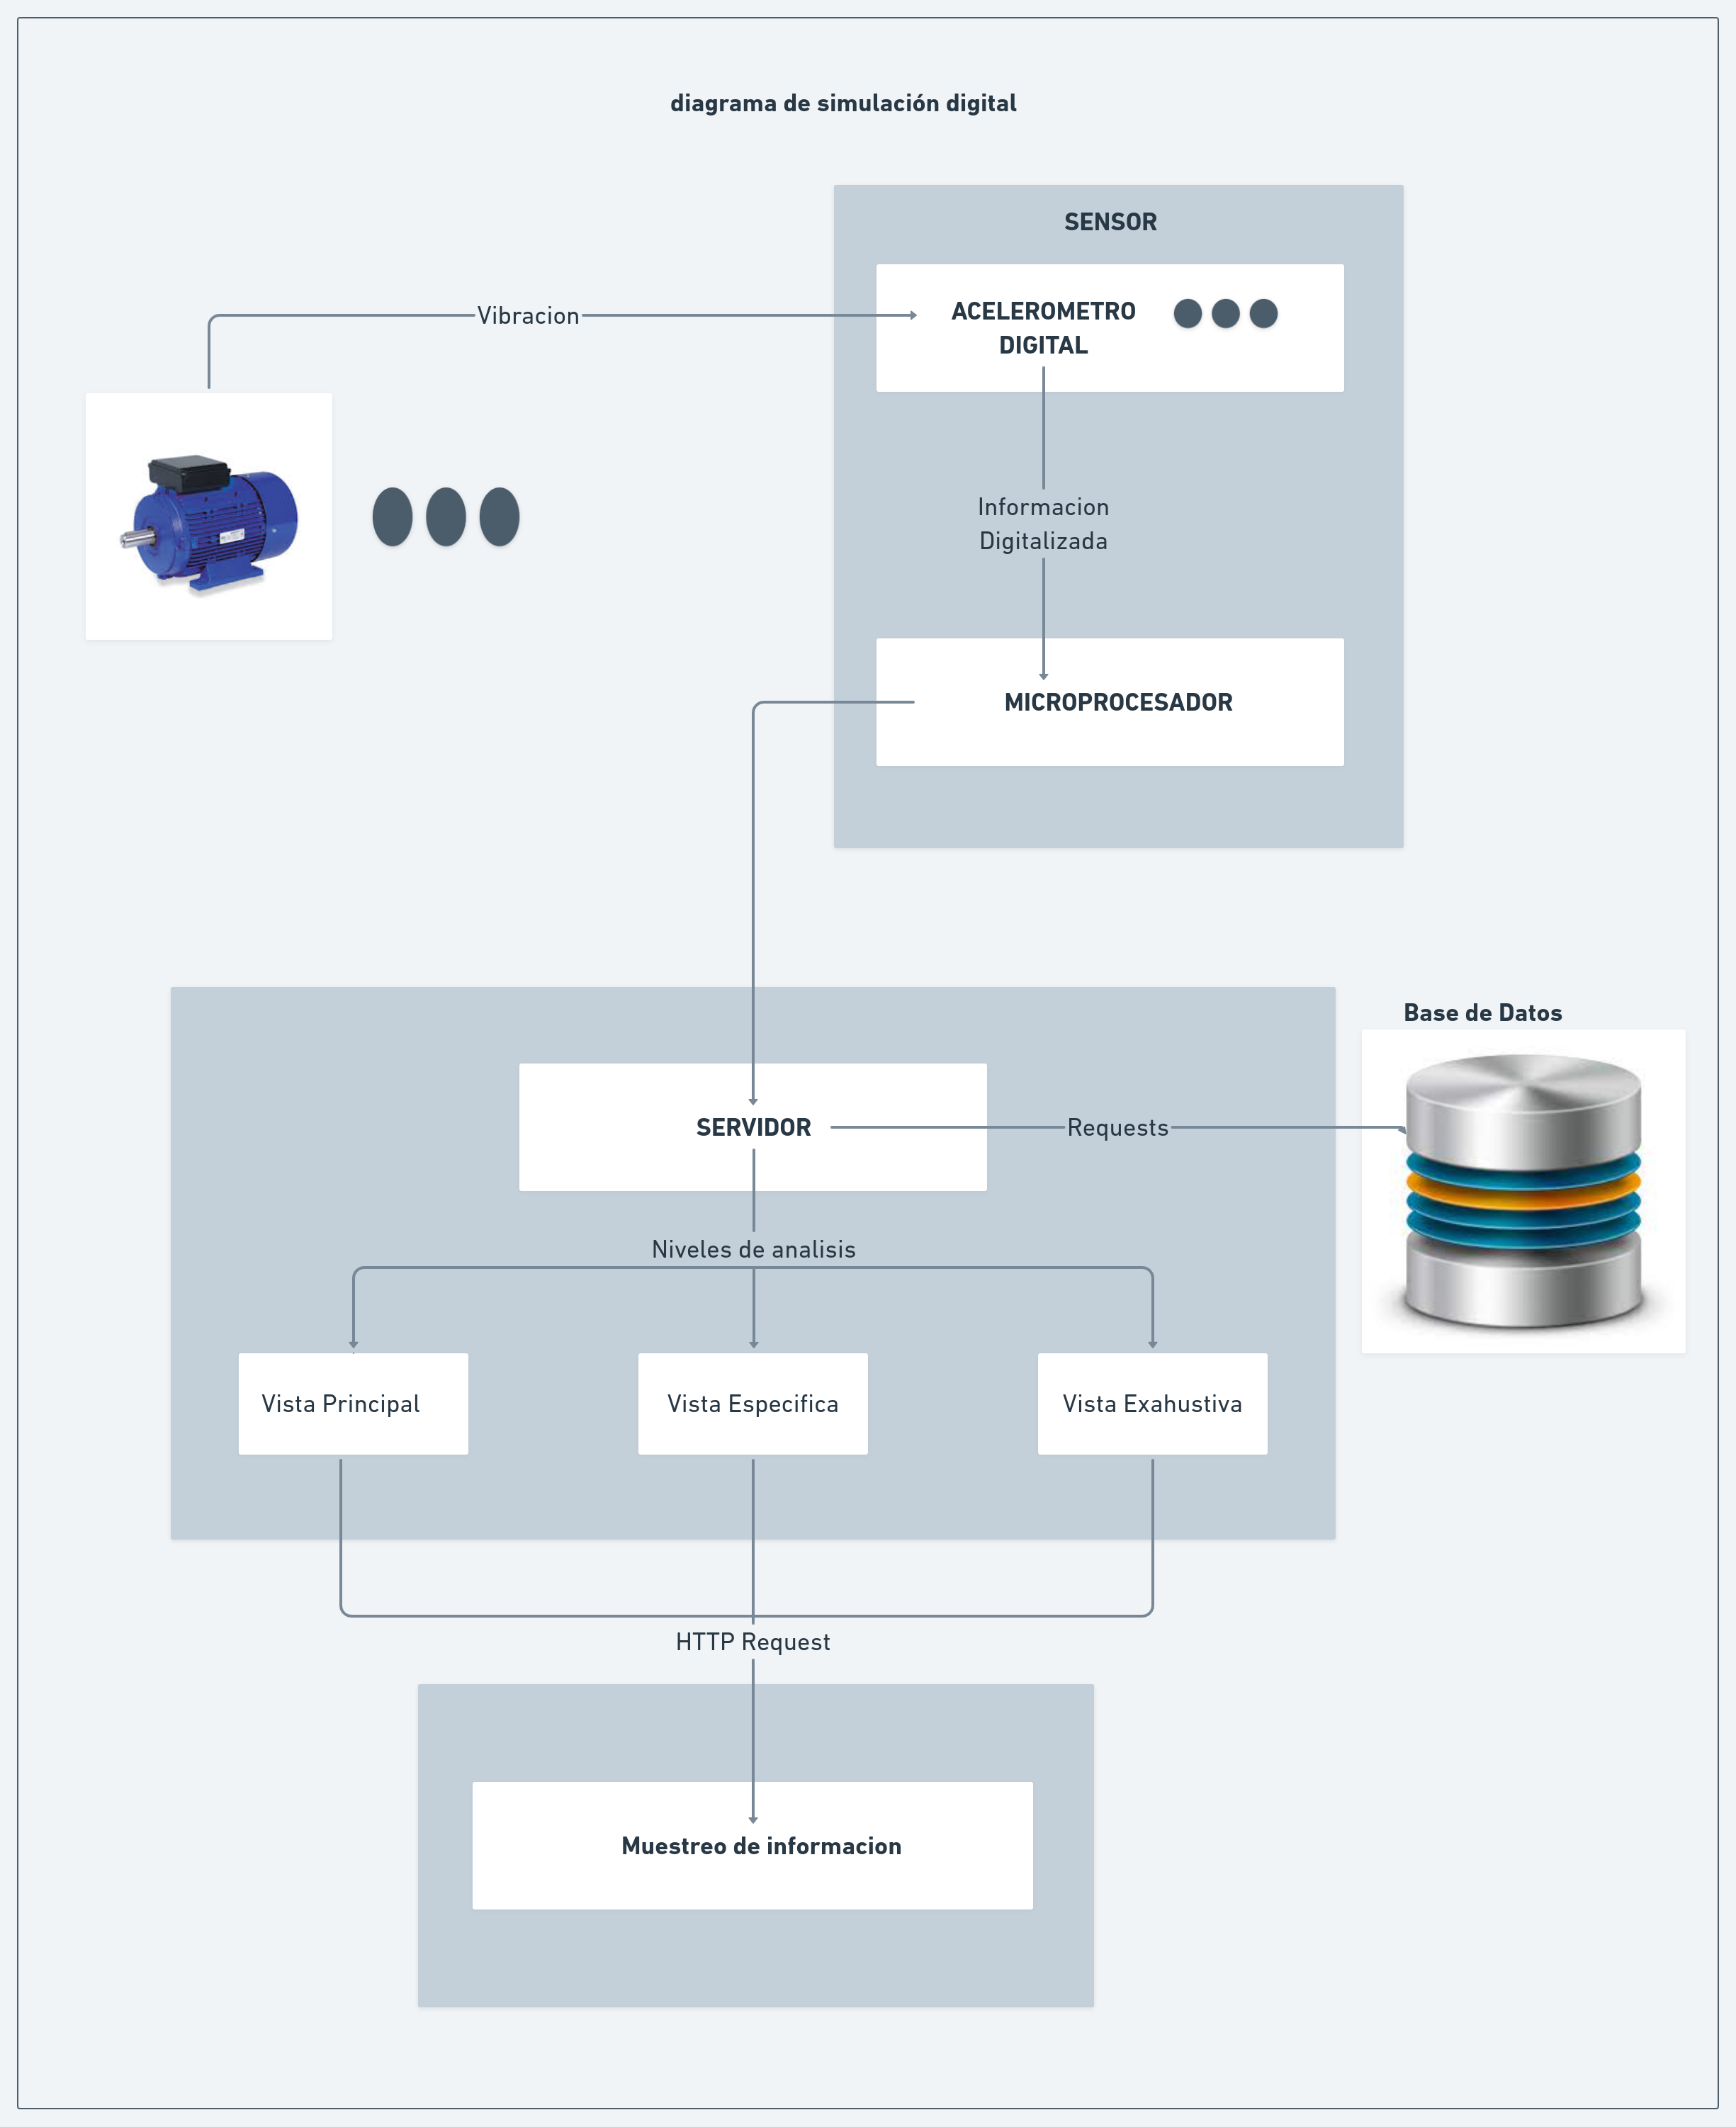
\includegraphics[width=15cm]{Diagrama_sensorica.png}
\caption{Diagrama de la simulación digital}
\label{fig:diagrama}
\end{figure}



	\subsection{Objetivos de la investigación}

\subsubsection{Objetivo general}
	\begin{enumerate}
		\item  Desarrollar la simulación digital del monitoreo de la vibración en motores eléctricos mediante un acelerómetro, con la finalidad de hacer diagnósticos predictivos.
	\end{enumerate}
	
\subsubsection{Objetivos específicos}

	\begin{enumerate}
		\item Justificar la escogencia de las herramientas y lenguajes a utilizar en las diferentes etapas que requiere la simulación. (José cortez y Gerardo Campos)

		\item Elaborar un análisis estadístico de motores con distinto grado de daño que establezca la distribución de la salida de acelerómetro digital. (José cortez)

		\item Elaborar una base de datos con la cual se establezcan el análisis  en simulación digital. (José cortez y Gerardo Campos) 
		
		\item Realizar análisis de fallas en frecuencia, a partir de la salida de la distribución del acelerómetro. (Gerardo Campos)

		\item Mostrar la información solicitada de acuerdo al nivel de análisis seleccionado. según sea: Vista Principal, Vista Específica o Vista Exhaustiva. (José cortez y Gerardo Campos)

		\item Comprobar los resultados de la simulación digital. (José cortez y Gerardo Campos)
	\end{enumerate}

	
	\subsection{JUSTIFICACIÓN E IMPORTANCIA}

Para prevenir las fallas mecánicas que ocurren en los motores, por el deterioro
y desgaste de los rodamientos, estos se deben tener bajo constante monitoreo
para poder efectuar un mantenimiento puntual que elimine dichos peligros. De
esta forma el mantenimiento predictivo es la clave para mejorar la vida útil,
funcionamiento y planificación de todo proceso especialmente a niveles
industriales, donde la cantidad de motores eléctricos es bastante elevada
por lo cual la automatización del proceso es crucial.

Sin embargo, dado los altos costos que implican realizar una automatización y
en especial a escalas industriales se suele hacer una simulación o una
emulación para estudiar y obtener el modelo más preciso, gracias a la facilidad
de manipular con mayor eficacia los diseños y conocer su comportamiento real
sin necesidad de construirlo, antes de realizar la implementación y todo el
proceso que esta conlleva.

Habiendo expuesto la importancia del mantenimiento como también la de realizar
simulaciones, se justifica el hecho de realizar el desarrollo del trabajo aquí
propuesto el cual permita emular el comportamiento y las salidas de un
acelerómetro, como también otorgar las herramientas necesarias para
realizar un mantenimiento predictivo, y de esta forma estudiar a
profundidad su estado actual como también su evolución histórica. Todo esto
sumado a las facilidades de portabilidad que ofrece un sistema Web, facilitando
la revisión constante sin las dificultades de los protocolos de acceso y
sanidad usuales en las plantas industriales.

	
\subsection{LIMITACIONES Y ALCANCES}
	En función de los objetivos planteados con anterioridad, se puede definir tanto las limitaciones como el alcance del proyecto.

\subsubsection{Limitaciones}
\begin{itemize}
	\item Recursos económicos impiden la adquisición de dispositivos para pruebas en motores reales.

	\item Disponibilidad de muestras, aunque se cuenta con una BBDD lo suficiente grande para cubrir el comportamiento de la vibración en motores, incluso de distinta potencia, esta es discreta y con intervalos de tiempo considerables entre cada muestra.

	\item Hardware utilizado, dado que para el desarrollo del servidor y la prueba del mismo se cuenta es con computadoras portátiles con bastante antigüedad, limitando de esta forma los recursos disponibles y por tanto la velocidad de desarrollo.

	\item La gran variedad de conocimientos. El conocimiento requerido es bastante amplio y ademas cubre áreas fuera del campo de la electrónica, como lo son probabilidad y mecánica de las cuales se cuenta con muy poco conocimiento previo, motivo por el cual se ralentiza el avance del proyecto.

	\item Las establecidas por el software de tercero, utilizado para incrementar la velocidad en el diseño del proyecto (parte gráfica).
\end{itemize}

\subsubsection{Alcance}
	El principal alcance de este trabajo es el desarrollo de una herramienta computacional para el análisis de la vibración en motores eléctricos; en función de esto:

	\begin{itemize}
		\item La herramienta computacional permite una vista general del estado de todos los motores en un espacio previamente delimitado y seleccionado (planta o piso) que se encuentren en la BBDD.

		\item La herramienta computacional muestra el estado especifico de un motor, seleccionado previamente por el operando, con todas sus características de forma mas detallada. 

		\item La La herramienta computacional genera un análisis en frecuencia de la vibración en un motor especifico para facilitar el estudio y la toma de decisiones del operando.

		\item Dados los puntos anteriores, el sistema consta de una Base de datos la cual permita su correcto funcionamiento y el almacenamiento de los valores históricos de cada motor.

		\item Se implementa un modelo estadístico para generar la información necesaria para el llenado de la BBDD  de la herramienta computacional y de esta forma evaluar su funcionamiento.

		\item Todo el sistema puede ser accedido de forma web para facilitar el acceso.

		\item no se contempla la construcción de hardware de ningún tipo.


	\end{itemize}



%***************************************************
%**********  Capitulo 2  ***************************
%***************************************************
%
%\subsection{solución}

%Para llevar a cabo lo expuesto anteriormente %en el planteamiento del problema
Para esto, se plantea la implementación de un sistema capaz de tomar datos de forma continua y enviarlos a un servidor el cual permita el almacenar, estudiar y muestrear la información en distintos niveles de profundidad, con respecto al análisis realizado.\\
Para esto se plantea una simulación digital, diagramada en la figura \ref{fig:diagrama}, que constara de un análisis estadístico para obtener las medidas típicas de un acelerómetro en motores eléctricos con distintos niveles de daños, esta data permitirá, después de ser almacenada en una base de datos y procesada, generar 3 niveles de análisis:\\
\begin{itemize}
\item La vista principal, permitirá observar una cantidad especifica de motores, simbolizando los existentes en una planta o piso, y su estado general.

\item La vista especifica, dará la información actual e histórica referente a un único motor previamente seleccionado.

\item La vista exhaustiva se refiere a un análisis en frecuencia de la vibración de un motor especificado con anterioridad, con la finalidad de permitir al operador o ingeniero encargado determinar la causa de las posibles averías.
\end{itemize}


Y finalmente, toda esta información y opciones se mostrarían a través de una pagina web para facilitar su acceso.

\begin{figure}[htb]
\centering
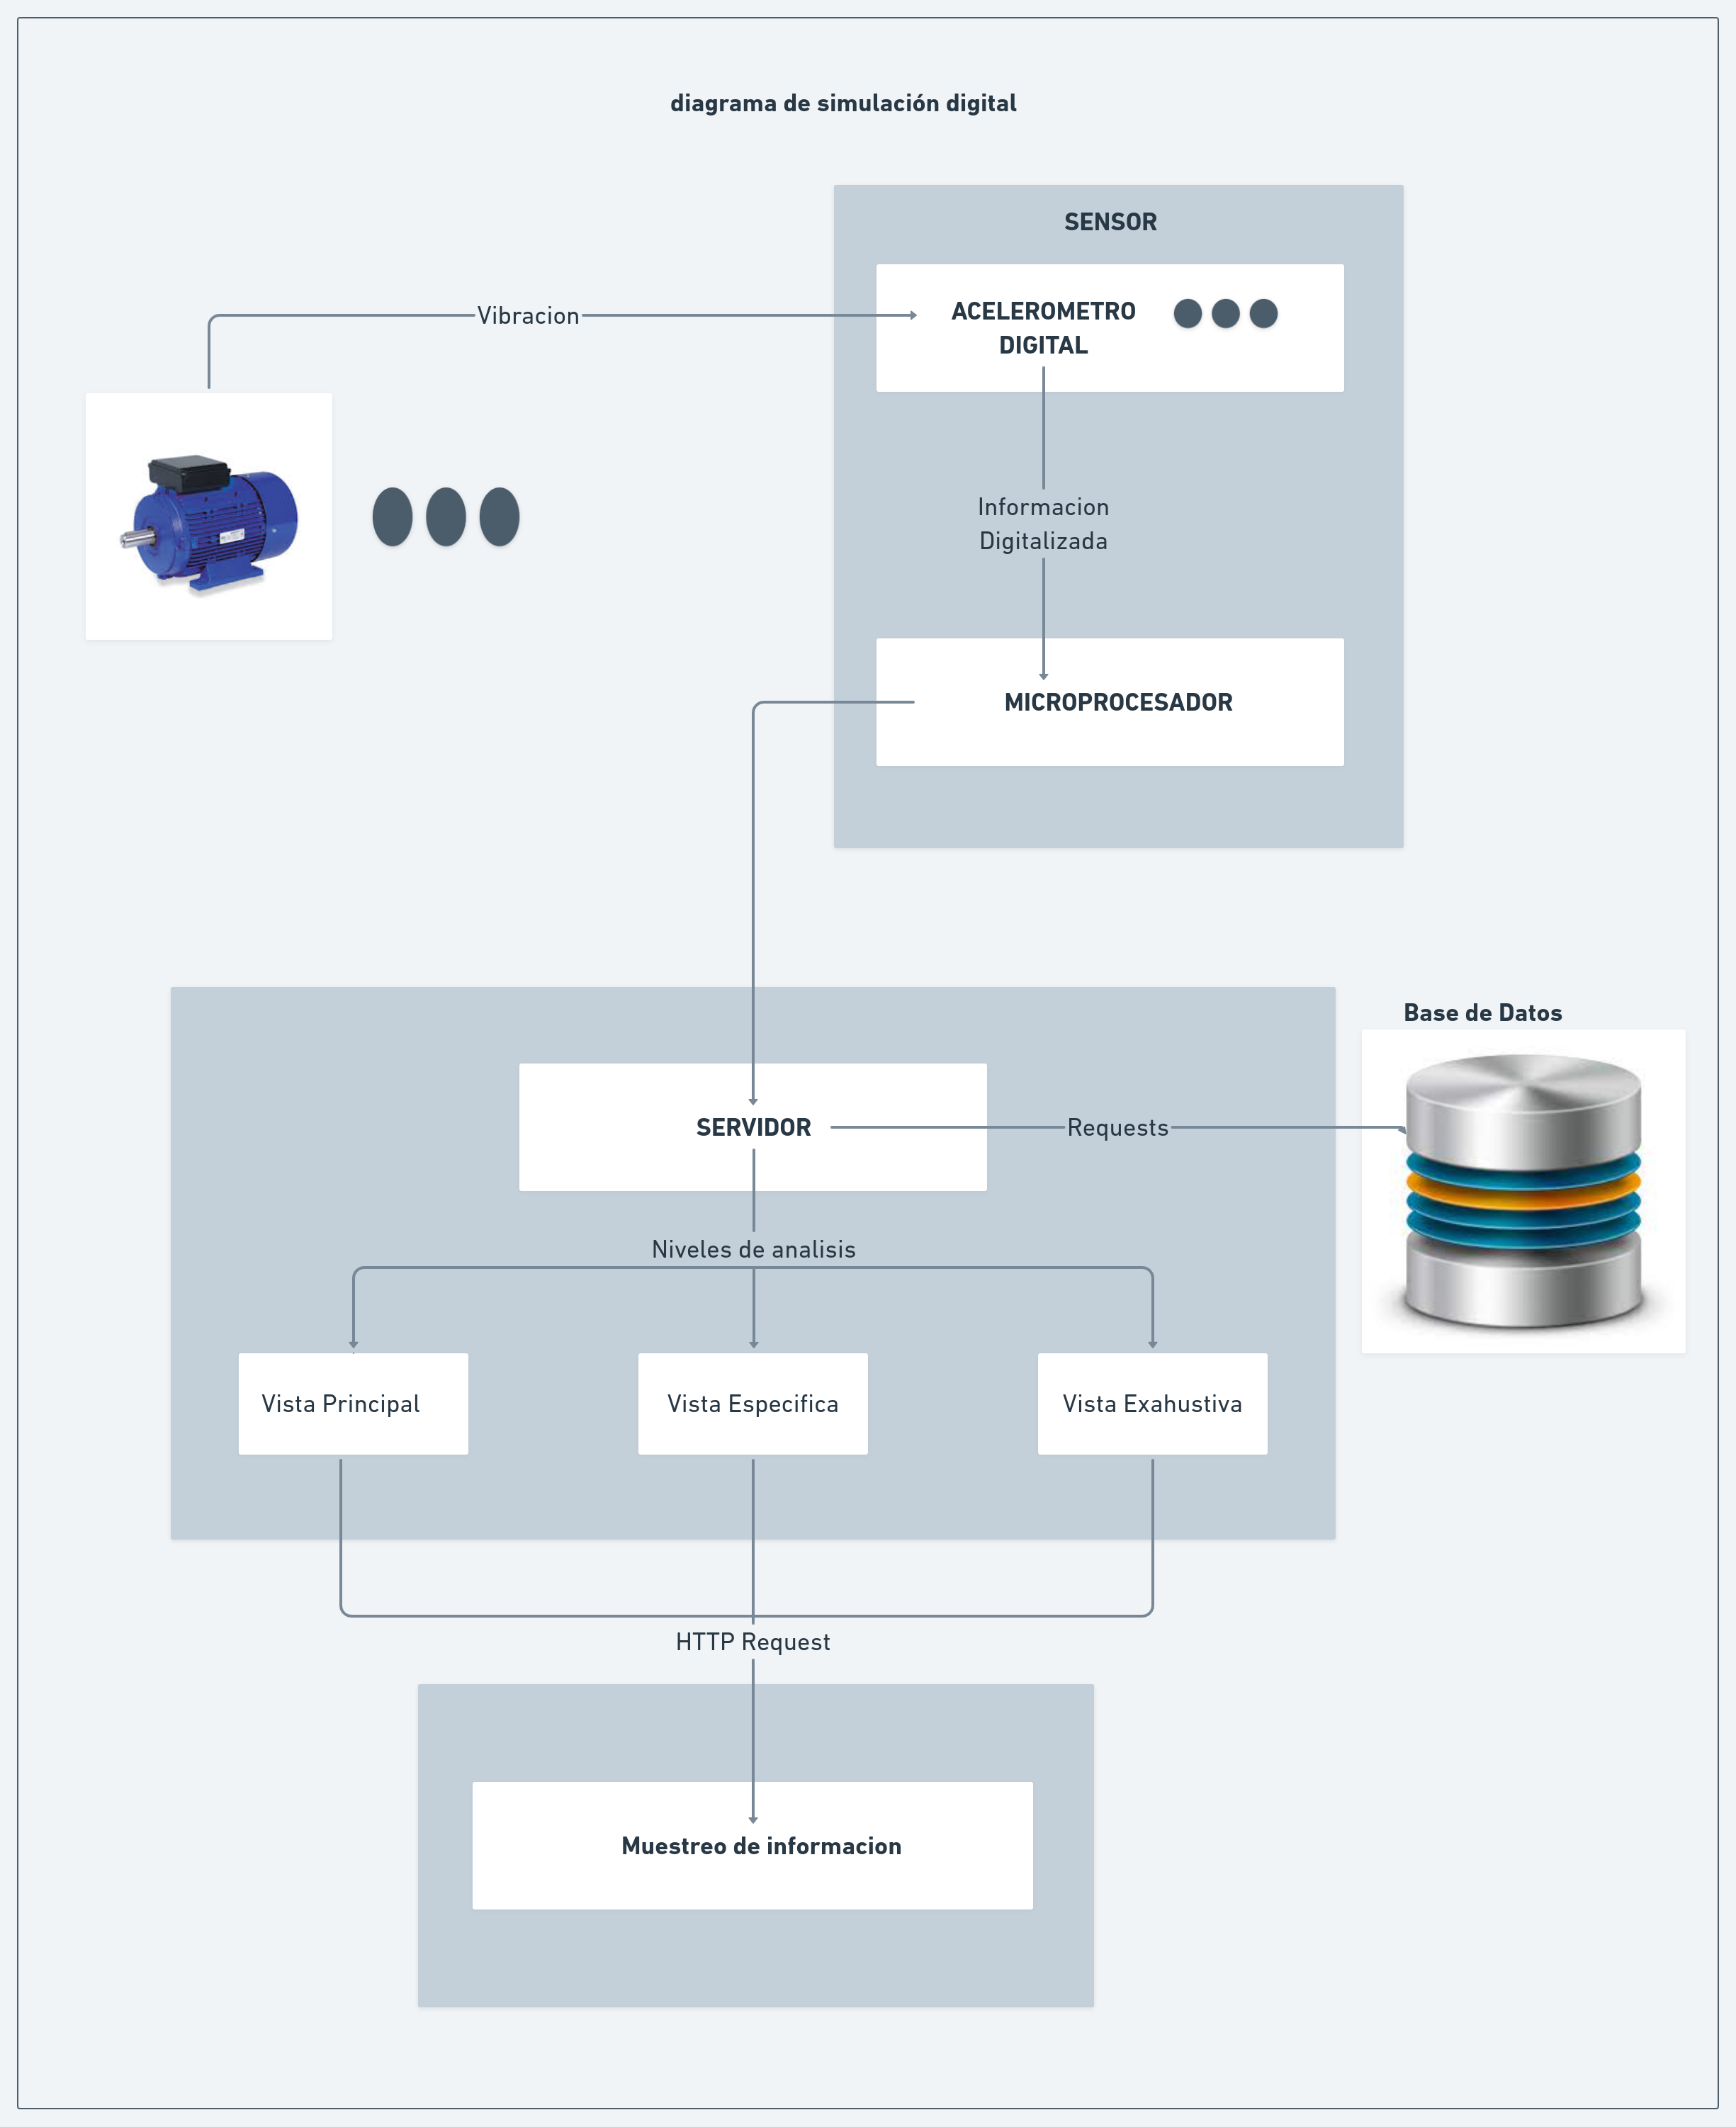
\includegraphics[width=15cm]{Diagrama_sensorica.png}
\caption{Diagrama de la simulación digital}
\label{fig:diagrama}
\end{figure}



	\thispagestyle{empty}

	\section{REVISIÓN BIBLIOGRÁFICA}


\subsection{ANTECEDENTES}

\textcite{Pinto} realizan una simulación de redes de sensores inalámbricos, con el fin de mejorar la detección de fallas de los sensores. Esta simulación fue realizada con Castalia un simulador de redes de sensores inalámbricos y el sensor usado fue un detector de luminosidad. Algunas de las razones que menciona el artículo de por qué fue escogida una simulación es debido a que realizar el experimento con sensores requiere un costo elevado de hardware y un estudio analítico no es efectivo, ya que la complejidad del sistema es muy grande. Este trabajo es de utilidad debido a que sirve como orientación a la elaboración de la simulación del sensor que generara el modelo estadistico.\\


\textcite{Ugwiri} Presentan un resumen de las técnicas más usadas actualmente en la detección de fallas en motores eléctricos mediante análisis de vibración, además de realizar un experimento donde se ponen a prueba algunos de estos conceptos. El propósito de este antecedente es el de apoyar la elaboración del modo de "vista exhaustiva".\\


\textcite{Koene} Elaboran un sensor de vibración inalámbrico de código libre llamado Memsio. Este dispositivo es alimentado por baterías y permite la adquisición de datos a alta velocidad por medio del uso de un acelerómetro microelectromecánico. Los autores mencionan que en la industria los sensores de aceleración más usados son los piezoeléctricos, debido a tener una mayor precisión y tolerancia al ruido, sin embargo los avances de los dispositivos microelectromecánico y su bajo costo hacen cada vez más factibles su uso para el monitoreo. Este antecedente muestra la tendencia de la reducción de precios de los sensores inalámbricos lo cual apoya al propósito del trabajo al hacer factible las redes de sensores.

	\subsection{MARCO TEÓRICO}

Esta parte del capítulo expone el contenido teórico necesario para la
realización de este proyecto. Esto incluye información sobre los motores
eléctricos,  análisis de la vibración, las herramientas computacionales, los
sistemas, y el modelado estadístico.

%https://es.wikipedia.org/wiki/Motor_el%C3%A9ctrico


\subsubsection{ Motores eléctricos}

De acuerdo a \Cite{Fraile}, un motor eléctrico es un dispositivo que
transforma energía eléctrica en
energía mecánica mediante la acción de campos magnéticos y están compuestos,
principalmente, por un estator (parte fija) y un rotor (parte móvil).
Existen dos familias principales de motores eléctricos las cuales, a su vez,
se subdividen en \textbf{motores de corriente alterna} como lo son los  motores
de inducción, síncronas, entre otros y los \textbf{motores de corriente continua}
como lo son los motores de escobillas,  sin escobillas, de imán permanente,
entre otros.

El motor más usado en el sector industrial, es el motor de inducción, debido
principalmente a su bajo costo y al poco mantenimiento que requiere para estar
completamente operativo, esto en particular es debido a su sencillo diseño
en comparación al de otros motores de igual potencia, ya que requiere  menor
número de componentes. Cabe resaltar que el segundo tipo de motor más usado es
el motor de corriente
continua, debido a que su control, en términos de torque y potencia, es mucho
mas sencillo para ciertos niveles de potencia.

También existen los motores síncronos, cuya construcción es similar a la de un
motor de inducción pero a su vez requiere de una fuente de alimentación externa
para el rotor, lo cual aumenta su costo, además de esto su velocidad es
constante, por lo tanto este tipo de motor es utilizado en aplicaciones
específicas. Como se mencionó anteriormente, existen otros tipos de motores,
pero son usualmente de menor potencia por
lo tanto su utilidad industrial es mucho más limitada.


\subsubsection*{Rodamientos}

Para que un motor pueda llevar a cabo la transformación de potencia debe rotar.
Esta acción es llevada a cabo por el \textbf{rotor}, el cual esta formado por un
eje que soporta un juego de bobinas envueltas sobre un núcleo magnético. Este
se encuentra suspendido por \textbf{rodamientos}, de forma que el movimiento y
las fuerzas producidas en la interacción entre las bobinas y el núcleo con los
campos magnéticos, producidos por el estator, puedan ser utilizados. Además,
los rodamientos, cuando se encuentran en buenas condiciones, permiten minimizar
el roce entre el eje y soporte, maximizando la transferencia de potencia.

Estos también son conocidos como \textbf{rolineras}, las cuales según
\cite{rodamiento},  son un tipo de cojinete,
un elemento mecánico diseñado para reducir la fricción entre un eje y los
elementos conectados al mismo. Existen muchos tipos de rolineras, sin embargo
su estructura se fundamenta en dos anillos concéntricos, algún elemento rotativo
como pueden ser bolas o rodillos, una jaula que se encarga de mantener los
elementos de rodadura separados además de guiados y un lubricante o un sistema
de lubricación.

Dado que son un elemento mecánico el cual es continuamente usado, sufre mucho
desgaste y es el elemento más propenso a dañarse, según los estudios realizados
por ~\textcite{Kammermann} el 59\% de las fallas son causadas por los rodamientos
y asimismo su principal falla es el desgaste, de igual forma se presentan
otras fallas estructurales. Y por estas razones es fundamental tener bajo continuo
monitoreo este elemento, esto se suele hacer a través de un análisis de vibración.


\subsubsection{Análisis de Vibración}

Como se explica en \Cite{wiki:Vibration}, la vibración, es el  movimiento
periódico de un cuerpo o medio
elástico, alrededor de un punto de equilibrio. En general podemos decir que una
vibración es un caso específico de una oscilación, cuando esta es de origen
mecánico.

Asimismo, se conoce como análisis de vibración, al conjunto de técnicas que permiten
obtener información de un equipo, a partir de sus vibraciones. Es una de las
técnicas más usadas en el mantenimiento predictivo de equipos mecánicos, debido
a que es un proceso poco invasivo y de bajo costo. El análisis de vibración
permite diagnosticar fallas de forma temprana, así como detectar señales
prematuras de desgaste.

Según Girdhar \Cite{Girdhar},  el análisis de vibración nos permite detectar las
siguientes fallas:

\begin{itemize}[noitemsep]

\item Defectos en los engranajes
\item Defectos en los rodamientos
\item Desalineamientos
\item Desbalances
\item Ejes torcidos
\item Excentricidad
\item Fallas eléctricas
\item Fuerzas hidráulicas o aerodinámicas
\item Mala sujeción en las piezas
\item Problemas en las correas de transmisión
\item Problemas de lubricación
\item Resonancia
\item Rozamientos en el rotor
\end{itemize}


\subsubsection*{Adquisición de datos}

Para realizar cualquier tipo de análisis, primero se deben adquirir datos y,
por regla general, mientras más datos se tengan y más precisas sean las
mediciones, mejores serán los estudios que se pueden realizar.


La adquisición de datos, según \cite{adquisiciondatos}, es el proceso de
realizar mediciones de fenómenos físicos
y registrarlos, en algún formato específico, para analizarlos posteriormente.
Cabe resaltar que en algunos casos es necesario hacer un acondicionamiento de
la señal, esto
implica modificarla controladamente al reducir o aumentar su amplitud además de
sumarle un nivel offset, voltaje continuo, para que cumpla requisitos mínimos
y pueda ser procesada por los siguientes circuitos.

Al momento de la adquisición de datos, se toman medidas de una señal analógica
la cual se convertirá al pasar por una serie de etapas y dispositivos en una
señal digital y se guardará en un formato deseado y en una unidad de
almacenamiento masivo (ROM, flash, etc.).
El primer paso en la toma de  datos comienza con el sensor, que es un
dispositivo el cual transforma la unidad física de interés, en una señal que
pueda ser procesada con mayor facilidad, luego esta se adecuará mediante un
circuito especializado a las características y requerimientos del sistema,
luego será procesada por un convertidor Analógico-Digital, el cual se encarga de
muestrear, retener y procesar la señal y, de esta forma, obtener una versión
digital de la misma, la cual se procesará o guardará mediante un software desde
una computadora.

En el caso de las vibraciones, los sensores más usados son los
acelerómetros.  Esto se debe principalmente a que tienen mayor ancho de banda
que los sensores de posición y los de velocidad, lo que les permite detectar
vibraciones de mayor frecuencia. Adicionalmente, dado que las vibraciones en los
rodamientos, por naturaleza, son de alta frecuencia y, como se mencionó anteriormente,
estos son componentes críticos en los motores eléctricos.
Estas características hacen al acelerómetro el sensor más utilizado para las
mediciones de vibración en motores eléctrico. Sin embargo,
en casos más especializados, como podría ser el análisis de vibración
de maquinaria de larga envergadura, son también usados los otros tipos de
sensores ya que sus características pueden facilitar el estudio.


\subsubsection{Acelerómetros}

Como se expone en \cite{Fraden}, un acelerómetro es un dispositivo capaz de
medir aceleración, no es
necesariamente la misma que la aceleración de coordenadas (cambio de la velocidad de
un elemento en el espacio), sino que es la correlación asociada con el fenómeno
de peso experimentado por una masa de prueba que se
encuentra en el marco de referencia del dispositivo.  Funciona mediante
la utilización de la segunda ley de Newton, \textbf{la fuerza resultante
ejercida sobre un cuerpo es proporcional a su masa por su aceleración}. Los
acelerómetros por lo general cuentan con una masa de prueba (también conocida
como masa sísmica), alguna especie de resorte y un marco de soporte que, a su
vez, puede funcionar como amortiguador. Debido a esto, los acelerómetros se
pueden modelar matemáticamente como un sistema lineal de segundo orden,
por lo que su respuesta en frecuencia posee un pico de resonancia.


\subsubsection*{Tipos de acelerómetros}

\begin{itemize}
    \item  Acelerómetros Capacitivos:

        Los acelerómetros capacitivos son uno de los modelos más sencillos
        capaces de medir
        aceleración, además de ser fácilmente utilizables y reproducibles en masa.
        Funcionan mediante una masa sísmica, dado que, al  experimentar una fuerza
        se desplaza con una aceleración proporcional a la fuerza aplicada.
        Si a la masa se le agregan unos resortes unidos a una carcasa, los resortes
        ejercerán una fuerza proporcional al desplazamiento de la masa generando un
        desplazamiento fácilmente medible.

        Este fenómeno se produce ya que estos efectos en conjunto al
        amortiguamiento producen un sistema lineal de
        segundo orden, este sistema matemático genera una salida en desplazamiento
        al aplicarse como entrada una fuerza
         Finalmente, al conectarse un sensor de desplazamiento, se observa
        la aceleración a la que esta sometido el instrumento.
        El sensor de desplazamiento más
        popular para este tipo de medidores es el capacitivo.

        En su mayoría los acelerómetros capacitivos vienen como dispositivos
        microelectromecánicos, \textbf{mems} por sus siglas en inglés, que son
        dispositivos
        fabricados con técnicas similares a las de fabricación de circuitos
        integrados, a su vez poseen componentes mecánicos microscópicos. Son los
        acelerómetros más populares en aplicaciones no industriales, sin embargo,
        en aplicaciones de bajo consumo, bajo coste o cuando las frecuencias con
        las que se trabajan no son tan altas, pueden ser usados a niveles
        industriales, ya que poseen múltiples ventajas como:

        \begin{itemize}[noitemsep]
            \item No requieren adecuación de la señal.
            \item Pueden comunicarse directamente con un microcontrolador.
            \item Su precio es económico.
            \item Son compactos.
        \end{itemize}


    \item  Acelerómetros piezoresistivos:

        Son, después de los acelerómetros piezoeléctricos, los más usados a nivel
        industrial. Su funcionamiento es similar al de los acelerómetros
        capacitivos, ante una aceleración de entrada se produce un desplazamiento
        de salida, más en este caso, estos están constituidos por una o varias
        galgas extensiométricas, una masa de prueba y unos resortes de soporte.
        La galga sujeta a la masa sísmica y, al esta recibir una fuerza, produce
        un desplazamiento proporcional a la fuerza aplicada, lo que deforma a
        su vez la galga extensiométrica lo cual se traduce como un
        cambio de resistencia en el sensor. La ventaja de los acelerómetros
        piezoresistivos es que pueden medir valores de voltaje DC lo que los
        hace útil en el estudio de impactos, son también usados en el
        análisis de vibración en el rango de mediana frecuencia.


    \item Acelerómetros piezoeléctricos:

        Según \cite{WeberPiezoelectricAT}, son el acelerómetro más usado en
        aplicaciones industriales ya que
        poseen características como:

        \begin{itemize}[noitemsep]
            \item Alto rango dinámico.
            \item Bajos niveles de ruido.
            \item Alta linealidad.
            \item Alto ancho de banda.
            \item Poco desgaste, ya que no poseen partes móviles.
        \end{itemize}


        Su construcción es bastante sencilla, se tiene disco de un cristal
        piezoeléctrico unido por dos terminales circulares, de forma similar a
        la de un condensador, y justo encima tienen una masa de prueba.
        Al experimentar una fuerza el cristal se deforma lo que produce una
        diferencia de carga y un voltaje proporcional a la fuerza aplicada.
        Como la aceleración de la masa de prueba es también proporcional a la
        fuerza aplicada, la aceleración del acelerómetro será entonces
        directamente proporcional al voltaje y la carga producida en el cristal.

\end{itemize}


\subsubsection{Procesamiento de señales}

Después de ser almacenada la información, debe ser estudiada, procesada, para lo
cual se utilizan una serie de herramientas, técnicas o software especializados
a cada necesidad. Este estudio se puede categorizar en dos ramas principales:

\begin{itemize}
    \item Dominio del tiempo, según \cite{wiki:DominioTiempo}, es un término
        utilizado para describir el análisis
        de funciones matemáticas o señales con respecto al tiempo, la sucesión
        de estados que atraviesa la señal de forma natural. Los estudios más
        comunes son en  \textbf{tiempo continuo} y en \textbf{tiempo discreto}.

    \item Dominio de la frecuencia, según \cite{wiki:DominioFrecuencia}, es un
        término utilizado para describir el análisis
        de funciones matemáticas, señales o movimientos periódicos respecto a
        su frecuencia, número de veces que sucede un evento en un periodo.
        Utilizan transformadas para llevar las funciones o señales del dominio
        del tiempo, base, al dominio de la frecuencia, deseado, la más famosa es
        la \textbf{transformada de Fourier}.
\end{itemize}


Gráficamente se suele entender el \textbf{dominio temporal} como la evolución
de una señal con respecto al tiempo, es decir su evolución natural, por otro
lado el \textbf{dominio frecuencial} muestra los componentes de la señal según
la frecuencia en la que oscilan dentro de un rango determinado.
En la figura \ref{Dominios} se observan ejemplos gráficos de señales en ambos
dominios.

	\begin{figure}[htb]
		\centering
        \caption{ Diagrama de los dominios temporal y frecuencial}
        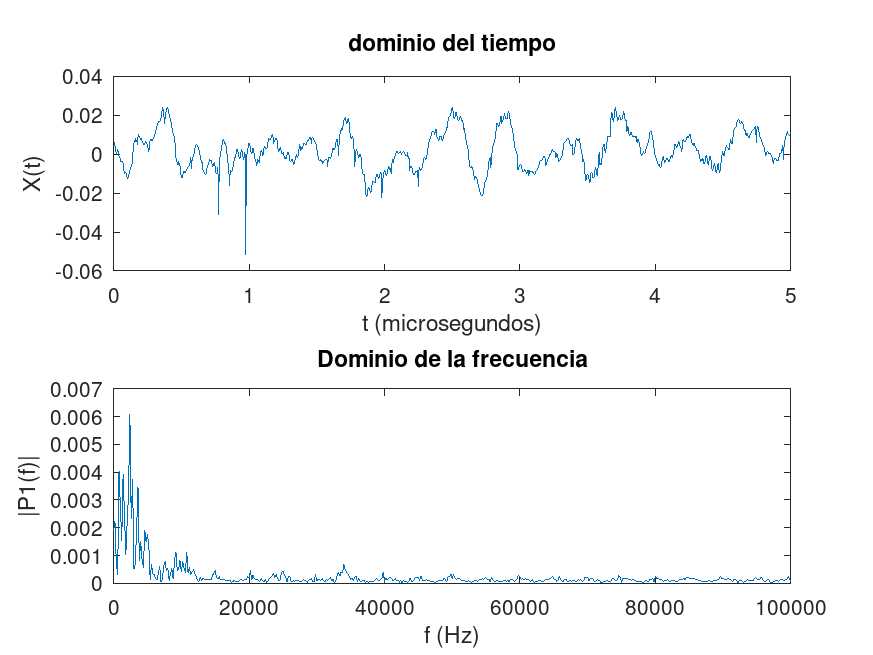
\includegraphics[width=\linewidth]{Dominios.png}
        Realizada con el Software Octave a partir de los datos de.
                \Cite{HUANG20181745}
        \label{Dominios}

	\end{figure}


El análisis en frecuencia suele ser más utilizado debido a que
la mayoría de las fallas poseen frecuencias características y, dado que en  el
análisis de frecuencia se descompone en frecuencias la señal, se facilita la
detección de fallas características, así mismo, la amplitud de la frecuencia es
directamente proporcional al nivel de la falla. Por lo tanto se obtiene un
espectro amplio del estado de la pieza.
Cabe resaltar que cuando las frecuencias son bajas o muy cercanas entre si,
se dificulta determinar e identificar alguna falla, suele suceder cuando se
estudia una falla o evento con frecuencia muy baja o muy cercana a la frecuencia
natural de la señal o elemento medido. En estos casos es mejor
usar un análisis en el dominio del tiempo que  facilita la
detección de las fallas.



\subsubsection{Herramienta Computacional}


Según \Cite{Herramienta}, una herramienta computacional puede ser definida  como
cualquier software,
sistema de integración, análisis o almacenamiento que  ayuda a los científicos
o usuarios a solucionar un problema específico en una determinada rama. Pueden
variar desde sistemas complejos como compiladores, algoritmos
e incluso sistemas operativos hasta herramientas como hojas de cálculos, sistemas
de oficina o medios de comunicación. Funcionan mediante la implementación de
técnicas y protocolos para solucionar problemas de forma iterativa o con una
secuencia de pasos concreta.

Siguiendo este orden de ideas, una gran cantidad de estas herramientas son
encontradas en la librería de información más grande del mundo, el Internet.
Todas comparten la peculiaridad de que son un \textbf{sistema} y,  por ende, pueden
ser accedidas con facilidad desde cualquier punto con un dispositivo capaz de
tener conexión a Internet y un navegador. Esta facilidad se debe a que un
\textbf{servidor} se encarga de hacer el procesamiento de la información y envía
el resultado con un formato específico, típicamente son  JSON, por \comillas{notación de
objeto de JavaScrip} el cual es un formato de texto sencillo para el intercambio de
datos, este se renderiza (proceso para generar una representación gráfica por
medio de programas informáticos) en una pagina Web.

\subsubsection{Sistema Web}

Los sistemas Web, de acuerdo a \cite{SistWeb1} y \cite{wiki:systemWeb}, o
también conocidos como aplicaciones Web son sistemas que
utilizan la tecnología Web y el Internet o Intranet para transmitir la
información y los
servicios a usuarios o otros sistemas/aplicaciones. Estos sistemas utilizan los
principios del hipertexto para renderizar la información en cualquier
navegador o \textbf{pagina Web} y el poder de los \textbf{servidores} para
almacenar y procesar la información. Por estas características son independientes
de cualquier plataforma o sistema operativo, además de  no requerir ningún
proceso de instalación, facilitando de esta forma el acceso, la gestión y la
rapidez de obtención de información.



\subsubsection*{Página Web}
Una página Web, como se explica en \cite{webpageMozila},  es un documento
accesible desde cualquier navegador con acceso
a Internet que puede incluir audio, vídeo, texto y sus diferentes
combinaciones.
Funciona al usar el protocolo HTTP, conocido usualmente como la Web, y una
estructura de hipertexto la cual permite redirigir, enlazar y estructurar el
contenido y lo hace fácilmente accesible desde un navegador Web.

Funciona gracias al protocolo HTTP, \comillas{Hypertext Transfer Protocol},
el cual es la base de cualquier intercambio de datos en la Web y un protocolo
de estructura cliente-servidor, esto implica que una petición de datos es
iniciada por el elemento que recibirá los datos (el cliente), normalmente un
navegador Web, y es cubierta por el elemento que envía los datos (el servidor).
Este protocolo comenzó siendo estático y dirigido usualmente a la transmisión de
texto pero se fue convirtiendo en más que eso y en la actualidad permite la
transferencia de documentos de todo tipo, scripts, vídeos, entre otros; a tal
punto que es fácilmente categorizado como el protocolo más usado en todo el
mundo, siendo incluso utilizado como sinónimo de Internet cuando es solo una
parte de él.

Debido a la invención de tecnologías como JavaScrip y AJAX hoy en día es
posible tener aplicaciones Web, que son programas junto a una interfaz gráfica,
que permite comunicarse con servidores que realizan la mayor parte del trabajo.
 Es posible el desarrollo de aplicaciones complejas que funcionen desde la
comodidad de dispositivos móviles. La Web permite, por tanto, facilidad a la hora
de transmitir información así como el poder acceder a cualquier contenido desde
cualquier dispositivo en cualquier momento.

La Web suele ser el método de acceso de muchas tecnologías y, si bien en la actualidad
el desarrollo Web usa el mismo estándar de tecnologías, el lado del servidor
contempla una variedad mucho más amplia, dado que cualquier aplicación que
pueda correr en un ordenador puede ser conectada a una interfaz Web. Teniendo
como limitante principal la latencia,  tiempo que tarda la información en viajar,
una interfaz Web es, para un usuario promedio, una solución cómoda y
accesible la cual  permite incluso  mayor comodidad y facilidad de acceso.


\subsubsection*{Servidor}

Un servidor Web, como lo define \Cite{servidor},  es un ordenador de propósito
específico que permite la
transición de datos a uno o múltiples clientes Web. Para esto, el dispositivo
debe de estar configurado para escuchar las solicitudes de los clientes en un
entorno red. Esto se logra mediante una aplicación externa o el uso de un
sistema operativo dedicado; almacena los archivos
necesarios para el procesamiento de información y los datos necesarios para
mostrarla, además, se encarga de distribuirla al usuario final.

Los servidores se suelen clasificar según su función y es común que cumplan más
de una función, o se encuentren más de un tipo en una red. Algunos de estos son
servidores de archivos, impresión, aplicaciones, DNS, \textbf{Web}, entre otros.
Actualmente, los servidores Web son los más abundantes en el mercado
y se caracterizan por alojar la información y los datos de los usuarios a través
de Internet o Intranet. Estos responden a las solicitudes de paginas Web u otros
servidores basados en esta tecnología.


\subsubsection{Interfaz de programación de aplicaciones (API)}
Interfaz de programación de aplicaciones es una forma de simplificar el diseño
de software al permitir el intercambio de información y funcionalidades de forma
rápida y segura. Como explica \cite{API} una API permite a las compañías y
desarrolladores abrir y expandir las informaciones y funcionalidades que poseen
con grupos externos de desarrolladores, compañeros de negocios e incluso departamentos
internos dentro de la misma compañía, esto permite separar los desarrollos y
trabajar de forma paralela ya que los desarrolladores no necesitan conocer la
implementación, simplemente la utilizan como interfaz para comunicarse con otros
productos y servicios.

Cabe resaltar que sin estas fuera imposible el desarrollo de muchas aplicaciones
populares. Una API funciona al ser un conjunto de normas que defines como se
comunicaran las computadoras o aplicaciones entre ellas, es decir, sirve como
una capa de abstracción entre el servidor y la aplicación.

\subsubsection{Modelo estadístico}

Un modelo estadístico, de acuerdo a \cite{modeloIBM}, es una representación
matemática que permite, mediante
ecuaciones, codificar información extraída de los datos y, de esta forma,
predecir el comportamiento de un sistema ante situaciones dadas. Funcionan
mediante  variables aleatorias, una o más variables de las cuales no
se tiene completa certeza de su valor o provienen de algún evento aleatorio.

Un modelo estadístico permite inferir ciertas características de un evento,
como qué tan probable es tal evento y cómo se distribuyen los valores de la
variable. Además se suele usar como primer paso en generar un modelo más
preciso o para la obtención de información cuando no se tiene suficiente,
es difícil su acceso o la naturaleza del
sistema es extremadamente compleja y dicha tarea es simplemente imposible.


\subsubsection{Lenguaje de programación}
Los lenguajes de programación pueden ser definidos, según \cite{ETAC} como
sistemas estructurados
que permiten a las personas o programadores interactuar y dar instrucciones a un
programa o software con la finalidad de lograr objetivos.

En la actualidad existen una gran cantidad de lenguajes de programación, algunos
desarrollados en la antigüedad que todavía desarrollan un papel importante en
los sistemas, como lo son C, C++, Java y otros más modernos como lo pueden ser
Go, Rust y Python.

Como se explica en \cite{javaTpoint}
Los lenguajes de programación suelen ser clasificados en bajo nivel y alto nivel,
haciendo referencia a la necesidad de un compilador o intérprete para poder ser
ejecutado por la computadora, siendo los de bajo nivel lenguaje de máquina o
ensamblador y los de alto nivel los lenguajes comúnmente conocidos, como
Python, Java, JavaScript, PHP, C++, Objective C, Cobol, Perl, Pascal, LISP,
FORTRAN, Go y Swift. Estos lenguajes de alto nivel se pueden subdividir
de acuerdo a la necesidad de un compilador (C,C++,Go, etc.) o de un intérprete
(Python, JavaScript, Ruby, etc.) en \cite{LenguajesCompiladosEInterpretados}, se
puede leer más de esto. Asimismo, existe otra pequeña subdivisión en el ``tipado"
del lenguaje, que es la necesidad de especificar el tipo de valor que una
variable o constante puede tomar, siendo estas posibilidades un tipado fuerte,
medio o débil, también llamados dinámico (débil) o estático (fuerte).


\subsubsection{Go}
Go es un lenguaje de programación creado en 2007 en google, específicamente por
Robert Griesemer, Rob Pike y Ken Thompson, su sintaxis es similar a la del lenguaje
C y tiende a ser dinámico como Python pero con un rendimiento equiparable a los
de C o C++. Como se especifica en su pagina y documentación oficial
\cite{GolangDocumentacion}: Go es un proyecto de código abierto (open source)
para hacer a los programadores más productivos, es un lenguaje expresivo, conciso,
limpio y eficiente con mecanismos de concurrencia (paralelismo) que permiten fácilmente
obtener el máximo rendimiento posible de las máquinas multinucleo y redes de máquinas
actuales, mientras permite una programación flexible y modular, además de un compilado
rápido con un recolector de basura (el lenguaje se encarga de liberar memoria
no utilizada).
Es un lenguaje compilado rápido y con tipado estático (las variables y sus tipos tienen que
ser definidos con anterioridad) que se siente como un lenguaje interpretado y
con tipado dinámico (variables modificables sin tipo definido, más sencillo de
escribir el código pero menos estructurado).

Adicional a esto, este lenguaje tiene un ecosistema de comunidades, librerías y
herramientas en constante crecimiento que facilitan el aprendizaje y el desarrollo
de código.

\subsubsection{Fyne}

Fyne es una de las librerías (conjunto de herramientas o paquete) más utilizado
en Go para el desarrollo de GUI, como se indica en su pagina oficial \cite{fyne}
el conjunto de herramientas de Fyne es una herramienta fácil de aprender, gratuita
y de código abierto (open source) que permite la creación de aplicaciones gráficas
para escritorios, teléfonos y más. Combina el poder y la simplicidad del lenguaje
Go con una cuidadosamente creada librería de widgets (miniaplicaciones o herramientas)
que hacen ahora más fácil que nunca la construcción de aplicaciones y su despliegue
a producción en todas las plataformas (sistemas operativos, ios, linux, windows, etc.)
y tiendas (windows store, google play, etc.).

\subsubsection{HTML}

HTML no es considerado un lenguaje de programación propiamente dicho por su
incapacidad de realizar acciones de lógica o aritmética, más específicamente y
de acuerdo a \cite{HTML},
es un lenguaje de enmaquetado (una forma de escritura que utiliza elementos
sintácticos para dar forma y estructura a la información escrita posteriormente
a un proceso de  compilación o interpretación por la máquina, otros ejemplos son
Latex y Markdown), específicamente un lenguaje de enmaquetado de hipertexto y es
el bloque más básico para la Web ya que define y estructura el contenido de la
misma.

``Hipertexto"\  se refiere a los enlaces que se utilizan para conectar la pagina
web con otras partes, ya sean de la misma pagina o paginas externas a la misma.
Estos enlaces son fundamentales en la Web ya que permiten la actualización y el
entrelazamiento de las paginas creadas por otras personas, esto permite
una participación activa el la\  ``World Wide Web".

HTML usa ``etiquetas"\  para dar información adicional  el texto, las imágenes,
el contenido y permitir
una correcta muestra del contenido, estos elementos sintaxicos son por ejemplo:
 <head>, <title>, <body>, <header>, <footer>, <article>, <section>, <p>, <div>,
 <span>, <img>, <aside>, <audio>, <canvas>, <datalist>, <details>, <embed>,
 <nav>, <output>, <progress>, <video>, <ul>, <ol>, <li>, entre otros.

 De esta forma, el mismo texto entre etiquetas distintas va a tener características
 visuales distintas, por ejemplo, <h1>Algo<h1> es un título, negritas y tamaño de
 fuente muy superior a <p>Algo<p> que sería un párrafo.


\subsubsection{CSS}

CSS al igual que HTML no es considerado un lenguaje de programación, por las mismas
razones, en cambio, como se describe en \cite{CSS} es una hoja de estilos en cascada,
un lenguaje utilizado para describir y dar estilo a documentos escritos en HTML o
XML, Esto lo consigue al describir como los elementos deberían ser mostrados en la
pantalla, papel, habla u otra tipo de multimedia.

Dado estas características CSS es una parte fundamental en el desarrollo Web, ya
sea en su versión para o con la inclusión de frameworks o librerías como lo son
Bootstrap o TailWind CSS.

Funciona mediante la especificación y modificación de las características en
entornos, etiquetas o elementos únicos, mediante identificadores, de un entorno
HTML o XML y por esto permite la modificación de los atributos.
Usualmente, en términos Web, se modifican tamaños de fuente, peso de la misma,
color de fondo o de fuente, márgenes, espaciado interno (padding), centrado,
entre otras cosas, y mediante la fijación de estas características a atributos
particulares se puede desarrollar un entorno gráfico completo, animaciones y
transiciones.

\subsubsection{JavaScript}

Como se describe en \cite{JavaScript}, este lenguaje de programación es liviano e
interpretado, débilmente tipado y es comúnmente conocido como el lenguaje estándar
de los scripts en las paginas Webs; sin embargo, también puede ser utilizado en
otros ambientes como a nivel de servidor y en aplicaciones multiplataforma.
JavaScript es un lenguaje basado en prototipos, multiparadigma, dinámico y de
ejecución en un silo hilo (no aprovecha la paralelización de los múltiples
núcleos) y soporta todo tipo de estilo de programación.

Sus estándares han ido evolucionando con el tiempo y son conocidos como
`` ECMAScript Language Specification"; comúnmente JavaScript corre del lado del
cliente y es utilizado para diseñar como las paginas web se ven o se comportan
ante algún evento especifico.

Al ser un lenguaje tan popular y común, posee una gran comunidad y una cantidad
muy significativa de ``Frameworks"  y librerías, facilitando su aprendizaje
y maximizando la cantidad de cosas que permite hacer. Entre las más conocidas
están: Node.js para el servidor, React, Angular y Vue para el cliente, además
existen librerías como JQuerry que facilitan el lenguaje.

\subsubsection{React}

React es una librería de JavaScript de código abierto diseñada por facebook y
lanzada por primera vez en 2013, como dice su documentación oficial \cite{React}
está diseñada para la construcción de interfaces de usuario, tiene una filosofía
de pagina única (singlepage) pero puede ser utilizada para desarrollar aplicaciones
de múltiples paginas. Esta librería tiene la característica de ser declarativa
y basada en componentes.

Como se mencionó anteriormente, React hace sencillo la creación de interfaces
de usuario al permitir la combinación de JavaScript con XML-HTML en ``jsx"\  dando
la posibilidad de devolver y renderizar HTML desde funciones con componentes
lógicos. Además, es completamente modular por lo que se pueden desarrollar
individualmente los elementos de la interfaz y juntarlos con total facilidad,
estos elementos son llamados componentes y utilizan todas las propiedades de
JavaScript y la manipulación del DOM (Document Object Model) para mostrar
y actualizar la información cuando es necesario.


\subsubsection{Python}

En su página oficial, específicamente en sus preguntas frecuentes
\cite{pythonDocs} se especifica que Python es un lenguaje de programación
interpretado, interactivo y orientado a objetos, este soporta muchos paradigmas
además del orientado a objetos, como lo son el procedimental y el funcional.
Python incorpora funcionalidades como módulos, excepciones, un tipado dinámico
y un muy alto nivel de dinamismo en los tipos de datos y clases, asimismo,
combina un poder computacional bastante alto con una muy clara sintaxis,
librerías, sistemas y compatibilidad con todos los sistemas operativos, además
de una facilidad para extenderse a los lenguajes C o C++.

Cabe resaltar que Python es completamente gratuito y tiene una gran capacidad,
dada su gran cantidad de librerías y frameworks, para cumplir muchas tareas,
como lo son estadística, sistemas webs, ciencia de datos entre otros.

\subsubsection{Django}

Django es un framework web de alto nivel de Python el cual fomenta un
desarrollo rápido, limpio y pragmático. Como se especifica en su documentación
oficial,
\cite{DjangoDoc} Fue creado para desarrolladores con experiencia que necesitan
un desarrollo rápido y completo en un proyecto web, con la finalidad de
permitir al programador desarrollar la aplicación propiamente dicha, es
completamente gratuito y de código libre.

Entre las características de Django son su gran velocidad para el diseño, gran
cantidad de extras y tareas adicionales fácilmente configurables
(autenticación, administración, etc.), seguridad (previene errores comunes
como SQL injection y  cross-site scripting-requests), versatilidad y facilidad
de escalabilidad.

Cabe destacar que Django permite la inclusión de librerías de Python para
cualquier ámbito y existen algunas específicamente diseñadas para facilitar el
desarrollo con este framework, por ejemplo Django rest framework, para la
creación de APIs desde el servidor de Django  y Django-cors-headers que permite
modificar y controlar el acceso de solicitudes a APIs desde clientes.

\subsubsection{Numpy}

Numpy es un paquete-extensión de Python diseñado para la computación
científica. Como se explica en su documentación oficial \cite{Numpy} es una
herramienta de computación numérica que ofrece una gran cantidad de  funciones
matemáticas, generación de números aleatorios, rutinas algebraicas de álgebra
lineal, transformadas de Fourier, el tratado de arreglos N-dimensionales,
vectorización e indexación de los mismos, todo esto a un gran rendimiento y una
facilidad notable de su uso . Además de todo esto, esta es una herramienta
gratuita de código abierto.

\subsubsection{Pandas}

Pandas es otra herramienta dedicada al cálculo numérico, es una herramienta
rápida, poderosa, flexible y de fácil utilización, además de código abierto,
utilizada para el análisis y la manipulación de datos, es creada en Python.
Entre sus características destacan su velocidad y eficiencia con objetos de
tipo DataFrame para la manipulación de la información, sus herramientas para la
lectura y escritura de información en distintos formatos, entre los cuales
destacan los formatos CSV, Excel, SQL DataBase y el HDF5, facilidad para la
mutabilidad, alineamiento, filtración y eliminación, inserción y separación de
datos, y una muy alta optimización con puntos de código críticos escritos en
Cython o C. Además de esto, otras características adicionales son expuestas en
su documentación oficial \cite{PandasDocs}

\subsubsection{SciPy}
SciPy es una librería-colección de algoritmos para la computación científica en
Python, como se explica en su sitio oficial \cite{Scipy}, esta desarrollado de
forma abierta en GitHub a traves del consenso y el trabajo de la comunidad
científica de Python y de la comunidad de SciPy. Esta herramienta provee estructuras
de datos y
algoritmos para optimización, integración, interpolación, problemas algebraicos,
ecuaciones, ecuaciones diferenciales, estadística, entre otros. Esta escrita
en lenguajes de medio-bajo nivel, como lo son Fortran, C y C++, haciendo sus
implementaciones bastante optimizadas y permitiendo el uso de código compilado
con la flexibilidad y facilidad de uso de Python.

\subsubsection{FastApi}
\cite{FastApi} define FastApi como un framework moderno y rápido, con alto
rendimiento, diseñado para
la construcción de APIs web en Python, tiene una versión mínima de 3.6. Sus
características principales son:

\begin{itemize}
    \item velocidad, equiparable con Node.js y Go haciéndolo
uno de los frameworks de Python mas rápidos actualmente.
    \item velocidad de escritura, permitiendo alcanzar un aumento en el desarrollo
        de hasta un 300\%.
    \item Facilidad, esta desarrollado para ser intuitivo, fácil, permitiendo
        reutilización y a su vez eliminando hasta un 40\% de los errores ( ``bugs")
        inducidos por humanos.
    \item Utiliza estándares de código abierto como lo son ``OpenApi"" y ``JSON Schema"".
\end{itemize}

\subsubsection{Octave}
Octave es un software originalmente escrito por John W.Eaton y muchos otros,
esto es debido a que es un lenguaje gratuito y constantemente incorpora
funciones o correcciones hechas por la comunidad. Como se especifica en su
documentación oficial \cite{octave}, es un lenguaje de programación de alto
nivel, orientado primordialmente a la realización de cálculos numéricos.
Permite el uso de una interfaz  o la terminal para resolver ecuaciones
lineales, no lineales, problemas numéricos además de conversiones y
transformadas matemáticas. Es completamente compatible con el lenguaje Matlab y
además puede ser utilizado como un lenguaje orientado a procesos.

Cabe resaltar que octave posee una gran gama de librerías o módulos escritos en
C++, C, Fortran entre otros lenguajes, y es completamente gratuito y
redistribuible.


\subsection{Git}
Es un software de control de versiones diseñado por Linus Torvalds pensado para
la confiabilidad y compatibilidad del mantenimiento de versiones de aplicaciones
especialmente útil cuando estas tienen un gran numero de versiones y archivos.
Como explica \cite{Git}, Git es un sistema de control de versiones distribuido,
gratuito y de código abierto, diseñado para manejar eficientemente tanto pequeños
como grandes proyectos de forma rápida y eficiente. Se diferencia de otros sistemas
por características como ramificaciones locales baratas, en términos computacionales
espacio y velocidad, múltiples flujos de trabajo en áreas de ensamblaje convenientes
(Permite trabajar tanto en clientes gráficos como en la terminal).

\subsection{GitHub}
GitHub es una plataforma para el montaje de  código y el control de versiones
basada en Git. Se utiliza para la creación de código fuentes ya que permite y
facilita la interconexión entre los programadores, como se explica en \cite{github}
GitHub  permite incrementar la velocidad del desarrollador, además de asegurar
cada paso, automatizar los espacios y flujos de trabajo, facilitando de esta
forma los patrones de desarrollo e integración continua y permitiendo la creación
de equipos de trabajo sin el impedimento de la ubicación geográfica.

\subsubsection{Digital ocean}

    
\subsection{Glosario}

\begin{itemize}
    \item motor electrico
    \item estator
    \item rotor
    \item torque
    \item potencia
    \item rodamiento
    \item Transferencia de potencia
    \item vibracion
    \item sensor
    \item adquisicion de datos
    \item ancho de banda
    \item acelerometro
    \item aceleracion
    \item posicion
    \item velocidad
    \item frecuencia
    \item acelerometro capacitivo
    \item acelerometro pizoelectrico
    \item acelerometro pizorresistivo
    \item Sistema de segundo orden
    \item dispositivo microelectromecánicos
    \item masa sísmica
    \item amortiguamiento
    \item Circuitos Integrados
    \item galgas extensiométricas
    \item rango dinamico
    \item voltajes DC
    \item voltajes AC
    \item ruido
    \item linealidad
    \item ancho de banda
    \item cristal pizoelectrico
    \item amplitud
    \item nivel offset
    \item señal analogica
    \item señal digital
    \item convertidor Analógico-Digital
    \item Dominio del tiempo
    \item Dominio de la frecuencia
    \item transformada de fourier
    \item componentes de una señal|
    \item Frecuencia natural
    \item herramienta computacional
    \item servidor
    \item pagina web
    \item Json
    \item Hipertexto
    \item internet
    \item intranet
    \item Web
    \item Pagina web
    \item Servidor
    \item javascript
    \item AJAX
    \item latencia
    \item Variable aleatoria
    \item Modelo estadistico
\end{itemize}





%***************************************************
%**********  Capitulo 3  ***************************
%***************************************************
	\thispagestyle{empty}

\section{MARCO METODOLÓGICO}

Como fue explicado en el primer capítulo, se pretende hacer una herramienta
computacional para el análisis de la vibración en motores eléctricos alimentada
mediante datos de una simulación digital. Partiendo de esto, se comenzará
con la definición de los siguientes aspectos.

\subsection{NATURALEZA DE LA INVESTIGACIÓN}

El presente trabajo es clasificado como Proyecto Especial, puesto que según
\textcite{Hernandez} lleva~a:

\begin{center}
    \parbox[ht]{13.5 cm}{Trabajos que lleven a creaciones tangibles,
    susceptibles de ser utilizadas como soluciones a problemas demostrados, o
    que respondan a necesidades e intereses de tipo cultural. Se incluyen en
    esta categoría los trabajos de elaboración de libros de texto y de
    materiales de apoyo educativo, el desarrollo de software, prototipos y de
    productos tecnológicos en general, así como también los de creación
    literaria y artística.}
\end{center}


\subsection{TIPO DE INVESTIGACIÓN}

De acuerdo con la clasificación el tipo de investigación de este trabajo se
cataloga como investigación aplicada, puesto que "persigue fines inmediatos y
concretos a través de la búsqueda de un nuevo conocimiento técnico con aplicación
inmediata a un problema determinado"\ \textcite{Velez}.

\subsection{FASES DE LA INVESTIGACIÓN}

En función de los objetivos específicos, se pueden definir las fases que conforman
la investigación:

\subsubsection{Definición de los requerimientos de usuario}
Esta fase tiene relación directa con la concepción del proyecto ya que fue el
planteamiento de los problemas y posibles soluciones, separación de vistas,
mecanismos de análisis, entre otros. Sin una concepción compleja de las estructuras
de datos y los lenguajes necesarios para elaborarla.
Como en todo proyecto, esta fase requirió de la interacción con el cliente (ingeniero
mecánico que propuso la idea) con la finalidad de puntualizar los requerimientos
mínimos necesarios para obtener una aplicación viable.

De esta manera, la primera fase ha constado de las siguientes actividades:

\begin{itemize}
    \item Selección de la cantidad de vistas óptimas para facilitar el estudio
        y el monitoreo de la planta, siendo esto decidido a 3, una vista
        \textbf{general} del estado de los motores en la planta, una
        \textbf{especifica} en donde se observa el comportamiento de un motor,
        una \textbf{exhaustiva} que añada información a la especifica, gráfica en
        el dominio de la frecuencia, agregada para mejorar la experiencia de
        usuario, por la demora necesaria para generar este estudio.
    %
    \item Definición de la estructura mínima necesaria para poder evaluar un
        motor, en términos de evolución histórica de la vibración, a base de
        una tabla histórica o gráfica (histórica).
    %
    \item Definición del tipo de transformada de Fourier a graficar para el
        análisis exhaustivo (por gustos y costumbres en la industria).
    %
    \item Entrega de una base de datos histórica con mediciones reales y esporádicas
        del estado de los motores en una fabrica.
    %
    \item Especificación de los parámetros a considerar para determinar un nivel
        básico del estado de un motor, en términos de velocidad y aceleración.
        Se debe resaltar que estos valores difieren de los establecidos a nivel
        teórico y recomendado en los estándares por factores inherentes a las
        empresas (malas instalaciones,
        utilización de bases artesanales, políticas de daños mínimos) los cuales
        amplían los rangos teóricos.
    %
    \item Selección de las unidades en las que se tomaran las medidas, siguiendo
        estándares, y siendo $\frac{mm}{s}(rms)$ para la velocidad y $g$ para la
        aceleración.
\end{itemize}

Es importante recalcar el hecho que los parámetros utilizados tanto
para el establecimiento de niveles de daño en el modelo estadístico como
en la vista general para distinguir el estado de los motores, son el resultado
empírico asociados a años de estudios del comportamiento de los motores en la
planta utilizada. Esto se tomo en consideración al momento del diseño y se puede
modificar, vía modificación de constantes en el código, los rangos de valores
en velocidad y vibración adecuados a los estándares de cada planta o ingeniero
que utilice el sistema.

\subsubsection{Revisión documental}
Relacionada parcialmente con los primeros dos objetivos de la investigación,
se baso en los estudios necesarios para poder tomar la decisión del tipo de modelo
y lenguajes a utilizar, el planteamiento de requerimientos para los
lenguajes, dada la gran variedad de posibilidades disponibles para las distintas
tareas a realizar; de esta forma, se pueden enumerar las siguientes actividades
realizadas:

\begin{itemize}
    \item Recolección de información de diversos lenguajes de programación.
    \item Estudio de estadística y los distintos modelos y distribuciones existentes.
    \item Estructurar los criterios y requerimientos mínimos para poder seleccionar
        las herramientas a utilizar.
\end{itemize}

\subsubsection{Análisis de la información}
Todavía una fase previa a la implementación pero relacionada al primer objetivo
de la investigación. Se procedió a analizar la información en la bases de datos,
comparar con los requerimientos mínimos por el cliente y estructurar mas detalladamente
tanto la nueva base de datos (creada posteriormente en MongoDB), los parámetros
necesarios para el modelo estadístico y la selección del tipo, orientado a una
distribución de probabilidad. Asimismo, se tomaron decisiones conforme a los
lenguajes utilizados y la estructura, de microservicios, que se utiliza en el
desarrollo. De esta forma, se distinguen los siguientes puntos en esta fase:

\begin{itemize}
    \item Organización de la información recolectada.
    \item Toma de decisión de los lenguajes y herramientas a utilizar, basada
        en los criterios previamente establecidos.
    \item Estructuración de los modelos para la base de datos.
    \item Justificación de las decisiones tomadas.
    \item Estructuración y separación de las tareas a realizar por los distintos
        microservicios (sensorica, Web, BBDD).
\end{itemize}

\subsubsection{Diseño del modelo estadístico}
Corresponde al segundo objetivo del trabajo pero guarda relación con los
objetivos 3 y 4. Se utilizaron técnicas de exploración de data para la
selección de las variables de interés así como la formulación de hipótesis y se
usaron pruebas estadísticas para seleccionar las distribuciones de probabilidad
que mejor modelan las variables de interés. Se realizaron las siguientes
tareas:

\begin{itemize}
    \item Limpieza de los datos.
    \item Análisis exploratorio de la data.
    \item Cálculo de estadísticos de interés.
    \item Cálculo de pruebas de bondad de ajuste para cada variable de interés.
    \item Selección de la distribuciones que mejor modelan cada variable.
\end{itemize}

\subsubsection{Diseño de las vistas para mostrar la información}
Este apartado guarda relación con los objetivos 5 y 6. Se trabajo en la
estructuración y diseño gráfico de las vistas, además de las funcionalidades
implementadas para poder ser creada la pagina Web. Las tareas realizadas
fueron las siguientes:

\begin{itemize}
    \item Toma de decisión en utilizar una aproximación multipagina (multipage app).
    \item Diseño básico, barra de navegación, encabezado y pie de pagina.
    \item Diseño de la vista General y su funcionalidad.
    \item Diseño de la vista Especifica y su funcionalidad.
    \item Diseño de la vista Exhaustiva y su funcionalidad.
\end{itemize}

\subsubsection{Implementación}
Dada la gran cantidad de tareas a desarrollar, la implementación se subdivide
en un gran grupo de tareas, con la finalidad de cumplir los objetivos 2,3,4,5,6
estas divisiones, y subdivisiones, pueden ser expresada de la siguiente forma:

\begin{itemize}
        \item Generación del modelo estadístico:
    \begin{enumerate}
        \item Inspección manual de la data.
        \item Limpieza de las variables de interés.
        \item Elaboración de histogramas para observar la distribución de los datos.
        \item Seleccionadas las variables velocidad horizontal, velocidad
            vertical y aceleración como variables para el modelo.
        \item Cálculo de correlación entre variables.
        \item Cambio de variables para reducir la correlación entre velocidad
            horizontal y velocidad vertical.
        \item Búsqueda de distribuciones que mejor modelan la data utilizando
            múltiples pruebas de Kolmogorov-Smirnov.
        \item Selección de distribuciones de Burr tipo III para modelar la
            magnitud de la velocidad y aceleración y distribución normal para
            modelar el ángulo.
        \item Calculo de parámetros de las diferentes distribuciones. Creación
            de API en FastAPI para servir los datos.
        \item Conexión de la API con el microservicio de Go.
    \end{enumerate}

    \item Elaboración de la base de datos:
        \begin{enumerate}
            \item Registro y creación del cluster en MongoDB Atlas.
            \item Creación de la base de datos ``tesis"\  y las colecciones
                ``MotorData"\  y ``MotoresInDB".
            \item Llenado mediante el servidor de sensorica.
        \end{enumerate}

    \item Microservicios de sensorica:
        \begin{enumerate}
            \item Creación de las estructuras de datos necesarias para manejar
                la comunicación con MongoDB.
            \item Obtención de un certificado y TLS/SSL.
            \item Creación del servidor Https.
            \item Creación de un cliente de sensorica, para facilitar la emulación
                de los sensores
            \item Implementación de las conexiones bidireccionales para el trafico
                de información.
            \item Creación del punto de conexión ``/sensormessage" para permitir
                la conexión de múltiples clientes y recibir la información.
            \item Creación del punto de conexión ``/exhaustive?idMotor\=identificador"
                para poder enviar la información de la vista exhaustiva.
            \item Intercomunicaciones internas en el servidor para poder comunicar,
                solicitar y verificar información entre los dos puntos de conexión.
            \item Verificaciones de seguridad y conexiones.
        \end{enumerate}

    \item Análisis en frecuencia:
        \begin{enumerate}
                \item Falta escribir
        \end{enumerate}

    \item Servidor Web:
        \begin{enumerate}
            \item Configuración para el envió de información estática
                (HTML, CSS, Js, imágenes).
            \item Creación del punto de conexión ``/" para la vista general.
            \item Creación del punto de conexión ``/especifica?IdMotor\= identificador"
                para la vista especifica.
            \item Creación del punto de conexión ``/exhaustiva?IdMotor\=identificador"
                para la vista exhaustiva.
            \item Creación de gráficas históricas.
            \item Solicitud de información y análisis en frecuencia, creación de
                la gráfica de frecuencia.
            \item Establecimientos de los puntos de conexión para las APIs que
                suministran las informaciones necesarias para las vistas (
                uno para cada vista).
        \end{enumerate}

    \item Muestreo de información, mediante las vistas:
        \begin{enumerate}
            \item Solicitudes de información a las APIs (fetch).
            \item Configuración de los valores y los niveles de daño.
            \item Establecimiento del motor svg con colores dependiendo del nivel
                de daño.
            \item Mecanismo de paginación y búsqueda para hacer mas fácil y agradable
                la UI.
            \item Creación de la vista general.
            \item Implementación de la tabla y la funcionalidad para exportar a
                excel.
            \item Solicitud y establecimiento de las imágenes-gráficas.
            \item Implementación de la vista especifica.
            \item Implementación de la vista exhaustiva.
            \item Diseño y estilizado mediante CSS.
        \end{enumerate}

    \item Interconexiones:
        \begin{enumerate}
            \item Interconexiones entre cliente y servidor de sensorica, mediante
                Http2 para poder establecer una comunicación bidireccional (full dúplex).
            \item Interconexión entre servidor de sensorica y API de modelo
                estadístico para información normal, grupo de 10
                mediciones de velocidad y aceleración por cada sensor.
            \item Interconexión entre servidor de sensorica y API del modelo
                estadístico para información exhaustiva, grupo de 1K de mediciones
                de aceleraciones, por sensor registrado al motor.
            \item Interconexiones entre el servidor de sensorica y la base de datos
                (MongoDB Atlas).
            \item Interconexiones entre el servidor Web y la base de datos (MongoDB Atlas).
            \item Interconexión entre servidor Web y servidor de sensorica, para
                solicitar la vista información asociada a la vista exhaustiva.
            \item Interconexión entre cliente Web y servidor Web para obtener
                información de archivos estáticos.
            \item Interconexión entre cliente Web y APIs del servidor Web para
                obtener la información referente a las vistas general, especifica
                y exhaustiva. Una interconexión y una API para cada vista.
        \end{enumerate}
\end{itemize}


\subsubsection{Comprobar los resultados}
Esta fase hace referencia al ultimo objetivo de la investigación: Comprobar los
resultados de la herramienta de análisis. Dada la extensión de la herramienta,
estas pruebas se pueden desglosar en dos niveles, resultados finales (evaluación
del análisis de la herramienta) y pruebas técnicas (también llamado testing).
Esto da origen a las siguientes tareas:

\begin{itemize}
    \item Testing: La elaboración modular del sistema permite  corroborar su
        funcionamiento de múltiples formas, dado que unas pruebas automatizadas
        escapan de esta investigación (por factores de tiempo y cantidad de pruebas
        y complejidad de las mismas a nivel de código) se toman pruebas manuales
        de sistemas e interconexión entre los mismos:
        \begin{enumerate}
            \item Prueba de no unicidad de la información, al haber múltiples
                clientes de sensorica enviando información sobre el mismo motor.
            \item Prueba de falla en la conexión de la base de datos.
            \item Prueba de solicitud de vista exhaustiva a un motor sin conexión
                establecida.
            \item Prueba de petición no completada en el cliente Web,
            información invalida (motor no existente) o error del servidor.
        \end{enumerate}

    \item Evaluación de resultados:
        \begin{enumerate}
            \item Corroboración del análisis en nivel de daño básico (vista general)
                que se ajuste a los parámetros requeridos por el cliente.
            \item Corroboración de las gráficas históricas.
            \item Corroboración de la gráfica de la transformada de Fourier.
        \end{enumerate}
\end{itemize}


% naturaleza de la investigacion
	
\subsection{RECURSOS}
\begin{itemize}	
	\item Computadoras portátiles.
	\item Documentación.
	\item BBDD de la vibración en motores eléctricos.
\end{itemize}	
	
\subsection{CRONOGRAMA DE ACTIVIDADES}

    Las actividades a realizar son las expuestas en la figura
    \ref{cronograma2}, y están pautadas para un
    lapso total de aproximadamente 13 semanas donde se planean 10 semanas de
    implementación:

%		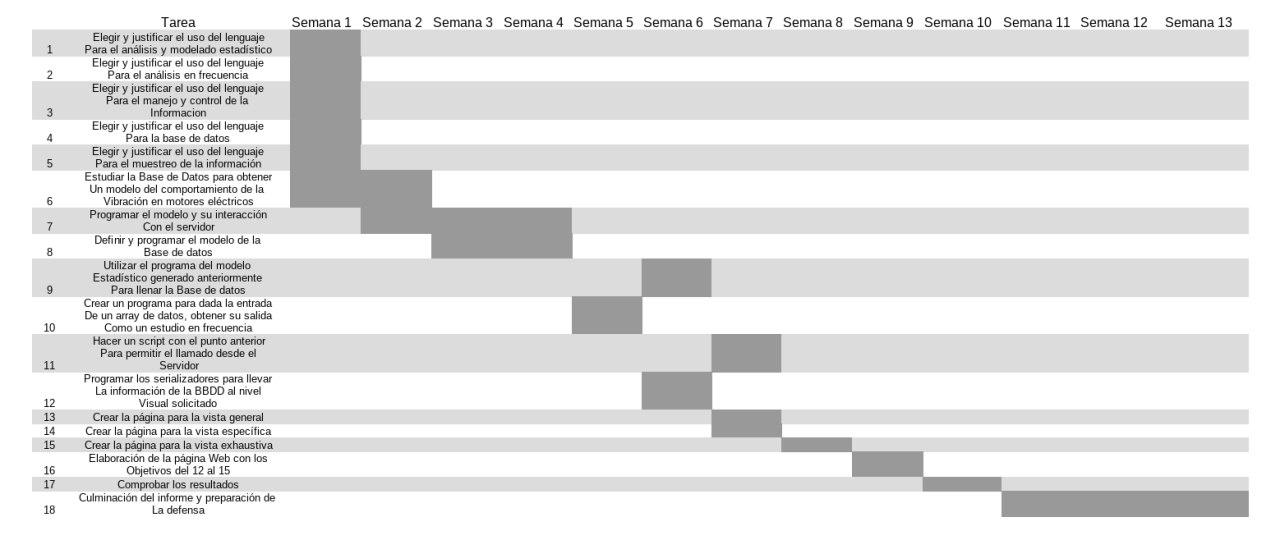
\includegraphics[trim= 2.5cm 0 -75 0,clip, width=1.2\linewidth  ]{diagrama_grant.jpg}
    \begin{figure}[htb]
		\centering
        \caption{Cronograma de actividades.}
		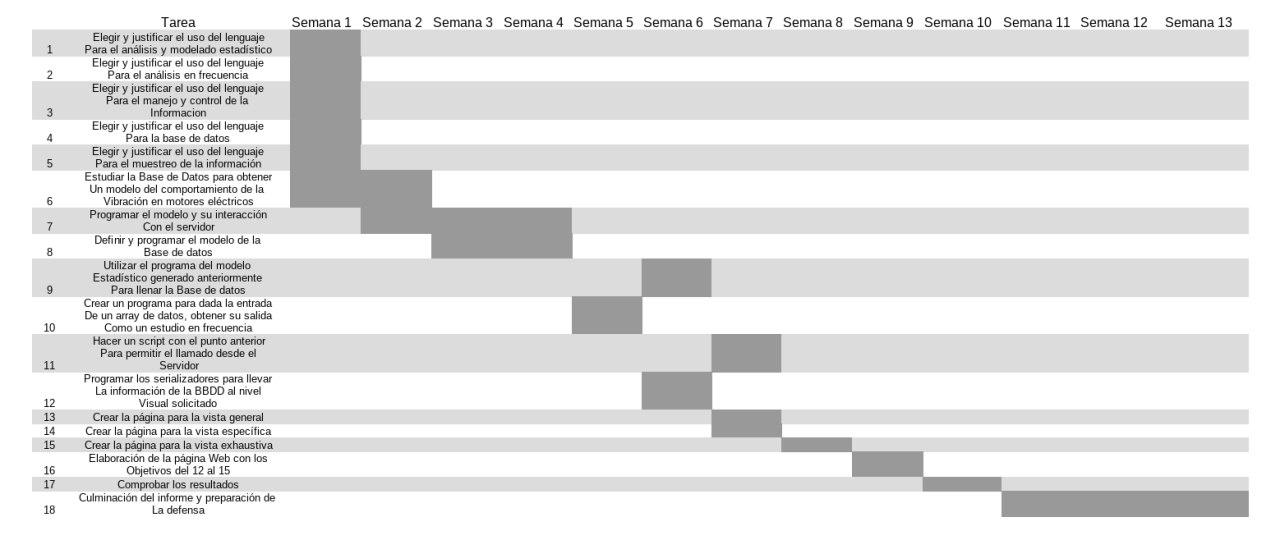
\includegraphics[ width=1.2\pdfpagewidth ,angle=270 ]{diagrama_grant.jpg}
		\label{cronograma2}
	\end{figure}



	\printbibliography[title={\centering{REFERENCIAS BIBLIOGRÁFICAS}}]
\end{refsection}

    \nocite{*}
	\printbibliography[title={\centering{BIBLIOGRAFÍA}}]

\end{document}
